\chapter{Contexte et problématique}
Le complexe d'accélérateurs du CERN est formé de plusieurs accélérateurs de particules. Chacun d'eux accélère un faisceau de protons issus d'une bonbonne d'hydrogène à une énergie supérieure. Le premier accélérateur de la chaîne est le Linac 2. Il permet d'accélérer les protons jusqu'à une énergie de 50MeV. Le faisceau résultant est par la suite injecté dans le \textit{Proton Synchroton Booster} (PSB), qui élève l'énergie des protons jusqu'à 1.4GeV. Le \textit{Proton Synchrotron} (PS) augmente l'énergie du faisceau jusqu'à 25GeV, suivi sur \textit{Super Proton Syncrotron}(SPS) qui augmente l'énergie jusqu'à 450GeV. Le dernier étage d'accélération est le LHC, lequel augmente l'énergie des faisceaux jusqu'à 4TeV. 

L'accélérateur étudié dans ce projet est le PSB, dans lequel on désire augmenter l'énergie des protons jusqu'à 2GeV.  La figure \ref{BOOSTER} présente un schéma de l'implantation du PSB. Le principe d'accélération d'une particules électriquement chargé repose sur les lois  fondamentales de la physique. Une équation générale résumant le phénomène étudié est présentée à l'équation \ref{eq1}.

\begin{equation}
\label{eq1}
\vec{F} = q\vec{\mbox{E}}(r,t) + q\vec{\mbox{v}}\times \vec{\mbox{B}}(r,t)
\end{equation}

L'alimentation concernée par l'étude n'agit que sur le champ magnétique (B), le champ électrique (E) étant un champ magnétique pulsé fournit par un autre système. Le champ magnétique est généré en utilisant des électroaimants, soit un noyau possédant une perméabilité relative ($\mu_R$) élevée dans lequel on injecte un champ magnétique au moyen d'un enroulement le fil avec un nombre de tours précis. On sait que le champ magnétique peut s'écrire comme une fonction linéaire du courant et de l'inductance des électroaimants, soit $B \approx \frac{N_{tour}I\mu_R \mu_0}{L}$. Si l'on désire fournir un champ magnétique variable au faisceau d'électrons, il est donc nécessaire d'alimenter les électroaimants avec une forme de courant variable. 

\begin{figure}[htb]
\centering
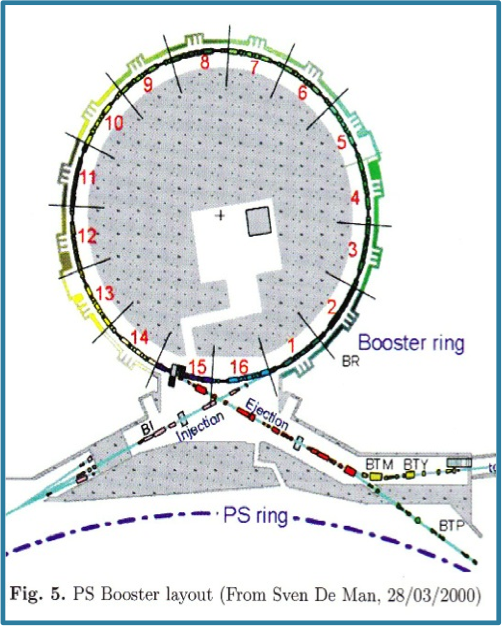
\includegraphics[scale=0.8]{BOOSTER.png}
\caption{Schéma de l'implantation du PSB au CERN}
\label{BOOSTER}
\end{figure}

\paragraph{AFE 3 niveaux NPC à 3 bras}Alimenter un faisceau d'électrons à des énergies élevées requiert beaucoup de puissance, sur un court laps de temps. De plus, au CERN, les cycles d'alimentation sont répétés de manière continuelle. Ce qui signifie que le réseau alimentant les électroaimants voit des impulsions de puissance élevée pendant de courte période, ce qui est relativement éprouvant pour un réseau électrique. Le CERN a opté pour un système comprenant un transformateur abaisseur, suivi d'inductances de lissage et d'un  convertisseur CA/CC actif (AFE) , permettant de contrôler l'échange de puissance active et réactive. L'AFE est un redresseur 3 niveaux \textit{Neutral Point Clamped} (NPC) à 3 bras, formé avec des IGBT de haute puissance. L'objectif de l'AFE est de maintenir la tension d'un bus CC, formé avec un banc de condensateurs d'une capacité de 0.3F, à 5kV avec une puissance moyenne de 2.7MW pendant un cycle. Le rôle du banc de condensateurs est de limiter la perturbation vue du réseau, causée par l'appel de puissance des électroaimants. L'AFE possède une fréquence de commutation de 1kHz, de manière à maximiser la durée de vie des interrupteurs. La méthode de commande employée pour les interrupteurs est une modulation de largeur d'impulsion (MLI), les formes d'ondes de tension, côté réseau, ont l'allure présentée à la figure \ref{fig_3L_Line_Voltage}. On remarque qu'il existe un total de 5 niveaux de tensions distincts pour la tension ligne-ligne, soit +VDC, VDC/2,0,-VDC/2 et -VDC. Le nombre plus élevé de niveaux est avantageux sur le plan de la qualité de l'onde. Aussi, les interrupteurs voient une tension maximale de VDC/2, ce qui est très avantageux sur le plan du dimensionnement.
\paragraph{DCP/DCN 3 niveaux NPC à 3 bras}L'alimentation des électroaimants est faite à partir du bus CC, sur lequel est rattaché un convertisseur CC-CC (onduleur) actif, ayant la capacité de contrôler l'échange de puissance active et réactive. L'onduleur est formé de 2 cellules, dénotées DCP et DCN, qui sont en soit des onduleurs 3 niveaux NPC à 3 bras, lesquelles sont rattachées aux électroaimants par le biais d'inductances de couplage. L'agencement des cellules permet de fournir une tension de $\pm$5kV aux électroaimants, ainsi qu'un courant allant jusqu'à 6kA. La forme de courant à fournir aux électroaimants est présentée à la figure \ref{fig_Iref} Les électroaimants sont modélisés par une inductance de 0.1H en série avec une résistance de 0.28$\Omega$. Les bras du convertisseur CC-CC ont une commande d'une fréquence de 333Hz, décalée d'un tiers de période. La figure \ref{fig_entrelacage} montre une représentation des formes d'ondes associées à une commande entrelacée d'un onduleur à k phases. Ce qui signifie que la tension vue à la charge est d'une fréquence de 1kHz. Cela est réalisé de manière à maximiser la durée de vie des interrupteurs et de minimiser les écarts de la température de jonctions. La tension moyenne maximale étant de 3kV, la puissance maximale consommée par les électroaimants pendant un cycle est de 18MW. La puissance moyenne pendant un cycle est de 5.4MW. L'excédent de puissance est fourni par le biais du banc de condensateurs, lequel subit une chute de tension pendant le cycle, de manière à limiter la puissance vue du réseau.Un schéma complet et simplifié du système est présenté à la figure \ref{fig_circuit_global}.

\begin{figure}[htb]
\centering
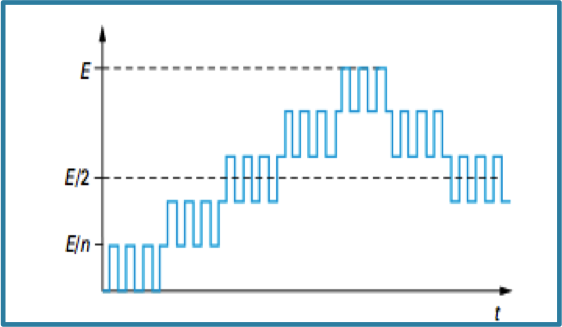
\includegraphics[scale=0.5]{fig/3L_Line_Voltage.png}
\caption{Allure de la tension ligne-ligne d'un convertisseur CA/CC 3 niveaux à 3 bras NPC}
\label{fig_3L_Line_Voltage}
\end{figure}

\begin{figure}[htb]
\centering
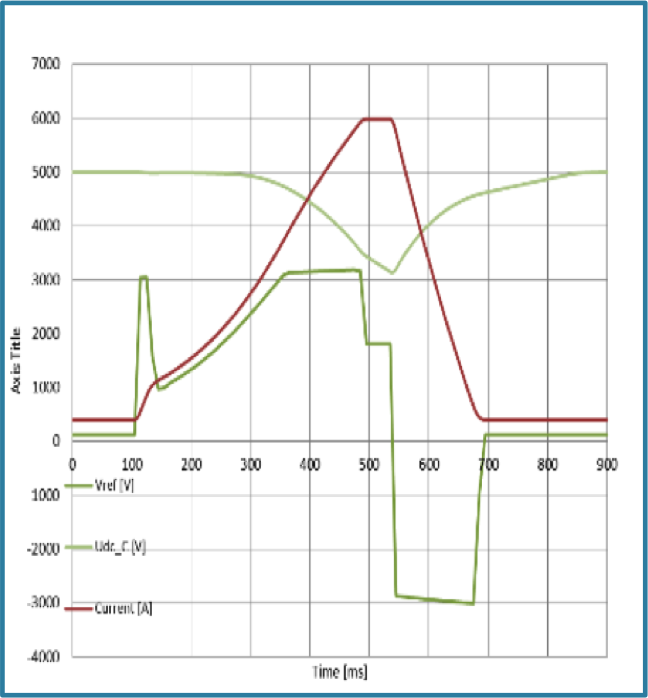
\includegraphics[scale=0.5]{fig/Iref.png}
\caption{Forme de courant et de tension à fournir précisément à la charge ainsi que la tension du bus CC en fonction du temps}
\label{fig_Iref}
\end{figure}

\begin{figure}[htb]
\centering
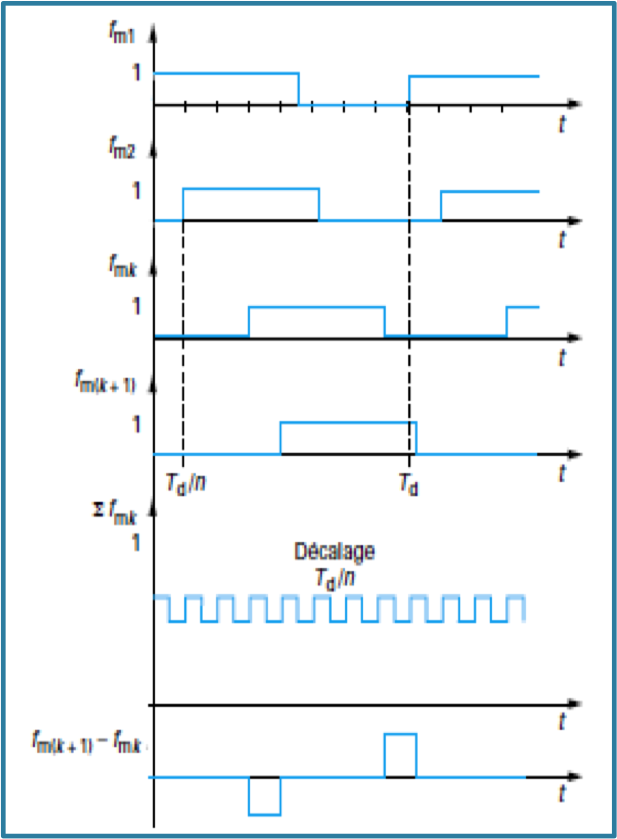
\includegraphics[scale=0.5]{fig/entrelacage.png}
\caption{Formes d'ondes type d'une commande entrelacée à k phases pour un convertisseur électronique}
\label{fig_entrelacage}
\end{figure}

\begin{figure}[htb]
\centering
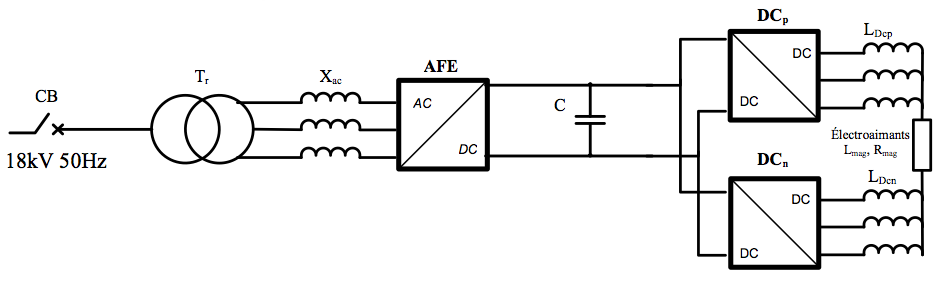
\includegraphics[scale=0.5]{fig/fig_circuit_global.png}
\caption{Schéma du circuit complet simplifié équivalent}
\label{fig_circuit_global}
\end{figure}

\paragraph{}Le client principal de ce projet est le laboratoire LEEPCI de l'Université Laval, lequel vise à obtenir une implantation sur 3 plateformes du système employé au CERN, d'une part afin de valider le comportement du système sous différentes plateformes et d'autre parts, afin de comprendre de manière théorique les choix pratiques effectués par la ingénieurs du CERN. Opal-RT est une compagnie œuvrant dans le domaine des simulateurs temps réels. Comme client et partenaire du projet, Opal-RT fournit une plateforme de simulation temps réelle qui permet de mettre en œuvre une validation additionnelle des modèles implantés sur SPS et PSIM. Les résultats obtenus du présent projet d'études visent à monter un document de support de formation pédagogique. Le schéma électrique complet de la simulation est présenté à la figure \ref{fig_circuit_electrique_complet}.

\begin{figure}[htb]
\centering
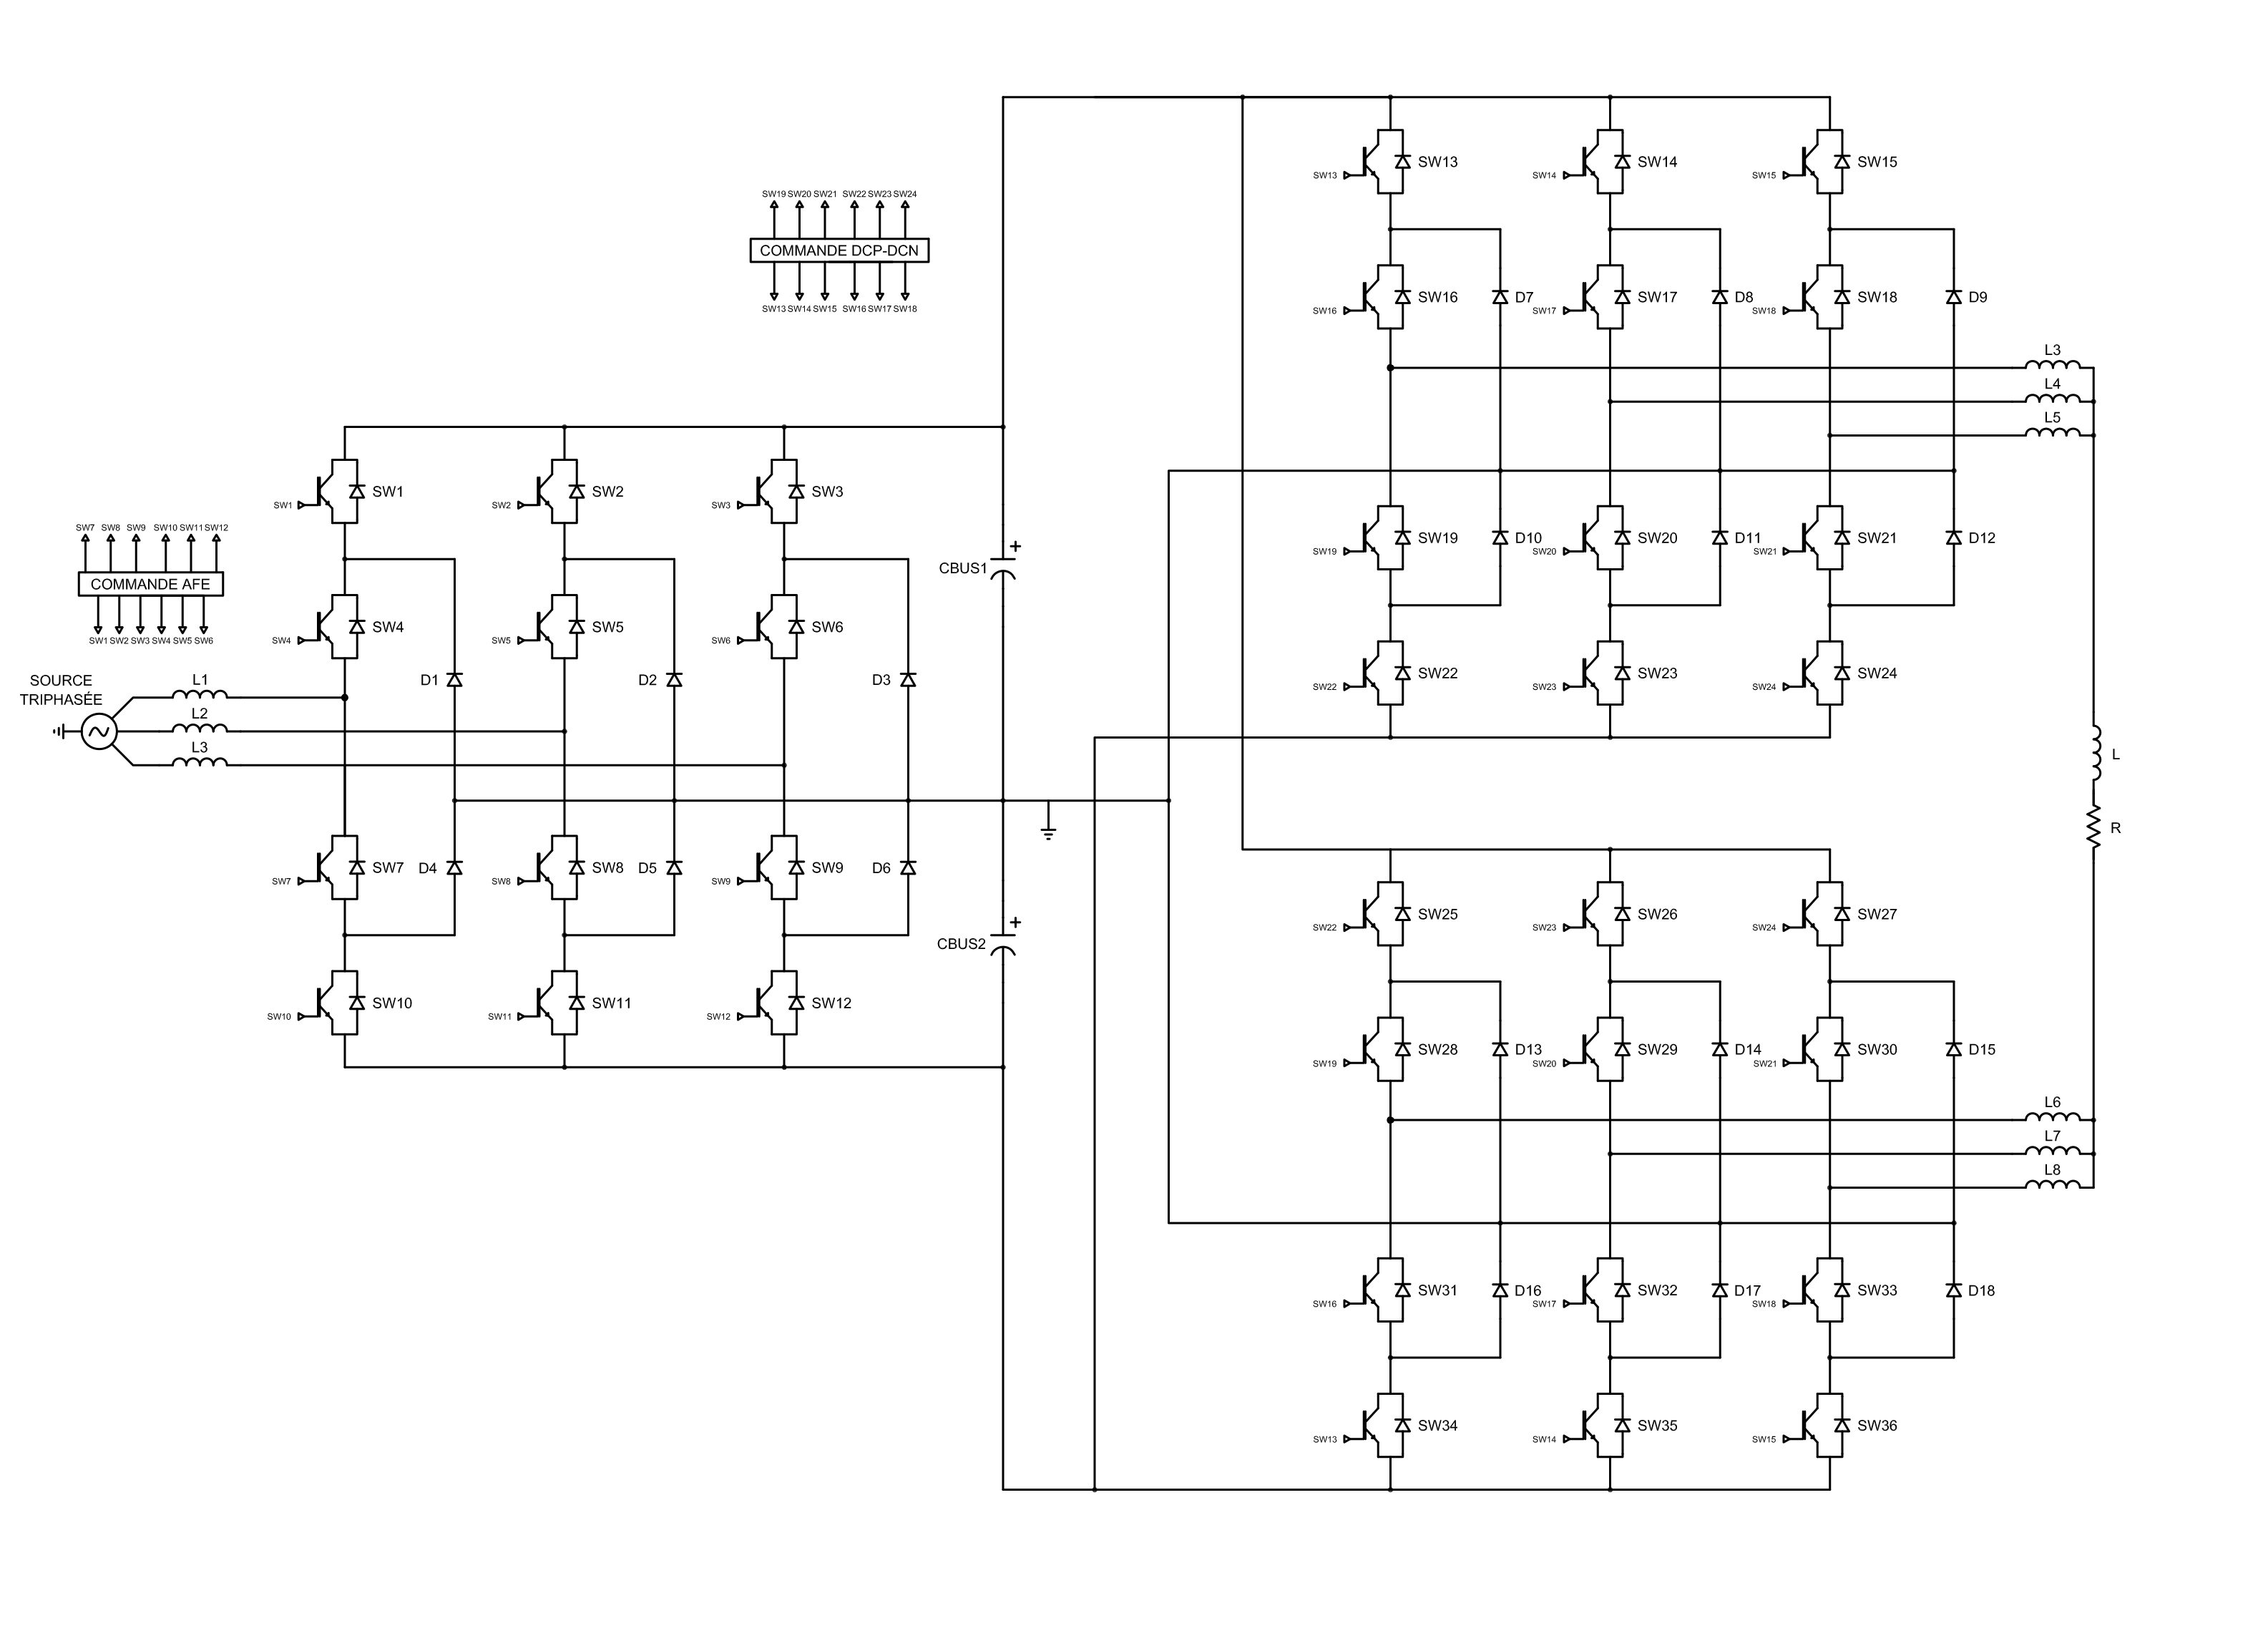
\includegraphics[scale=0.65]{fig/AFE_3L_RC_DCP_DCN.png}
\caption{Schéma électrique complet du système à implanter.}
\label{fig_circuit_electrique_complet}
\end{figure}
